\documentclass{beamer}
\usetheme{Singapore}

\usepackage{dcolumn} %use for aligned decimal points
\usepackage{booktabs} %use for toprule etc.
\usepackage{hyperref}
\usepackage[backend=biber,style=bwl-FU,url=false,doi=false,eprint=false]{biblatex}

\title{Beamer Final Assignment DTFF}
\author{S. Kim, M. Kiefer, V. Khmarskyi, B. Clays}
\institute{University of Zürich,}
\titlegraphic{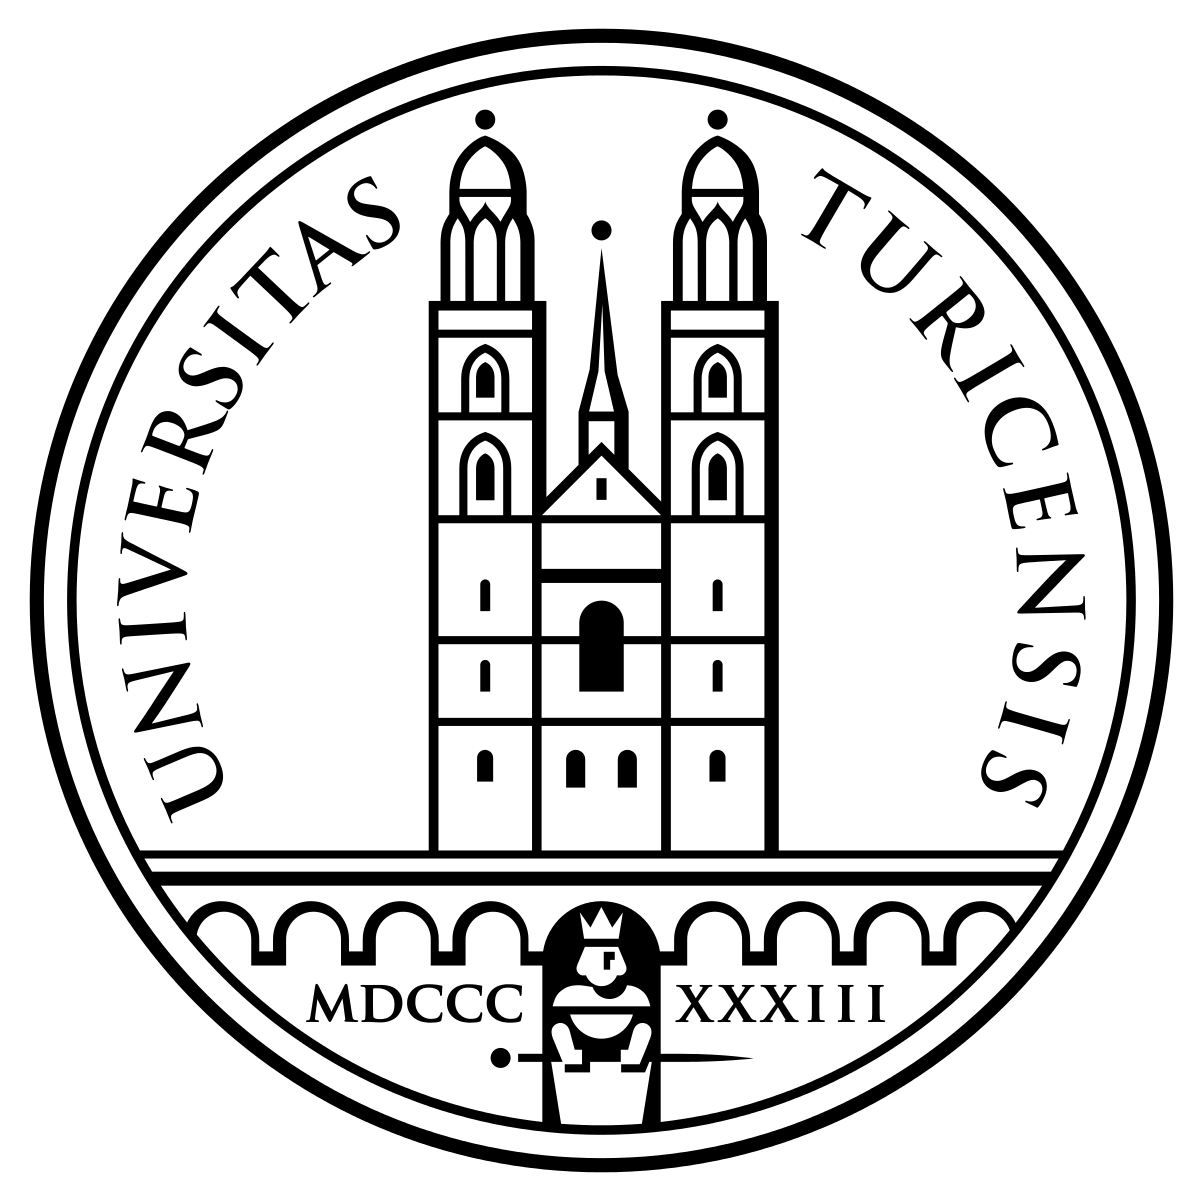
\includegraphics[width=2cm]{uzh.png}}
\addbibresource{finalassignment.bib}


\begin{document}

\begin{frame}
\titlepage
\end{frame}

\begin{frame}{Table of Contents}
\tableofcontents
\end{frame}

\section{Introduction}

\begin{frame}{Short lists}
\framesubtitle{2 summations}

Here is an itemized list of some courses:
\begin{itemize}
    \item Digital Tools for Finance
    \item Financial Engineering
    \item Stress Testing of Banks
\end{itemize}

\bigbreak

Here is an enumeration of some stuff:
\begin{enumerate}
    \item First thing
    \item Second thing
    \item Third thing
    \item Test my thing
\end{enumerate}

\end{frame}

\begin{frame}{This frame contains Pythagoras' theorem}
\framesubtitle{A very useful theorem}

\begin{theorem}
In a right-angled triangle, the square of the hypotenuse side is equal to the sum of squares of the other two sides.
\end{theorem}

\end{frame}

\section{Interesting equations}

\begin{frame}{Some statistics equations}
\framesubtitle{2 widely applicable equations}
\begin{block}{Unbiased Sample Variance}
    \begin{equation}
       \sigma_X^2 =\frac{1}{n-1}*\sum_{i=0}^n (X_i-\overline{X})^2
    \end{equation}
\end{block}


\begin{block}{Correlation}
    \begin{equation}
  r =
  \frac{ \sum_{i=1}^{n}(x_i-\bar{x})(y_i-\bar{y}) }{%
        \sqrt{\sum_{i=1}^{n}(x_i-\bar{x})^2}\sqrt{\sum_{i=1}^{n}(y_i-\bar{y})^2}}
\end{equation}
\end{block}

\begin{block}{A little new mathematical stuff}
  \begin{equation}
      \oint_{C} \vec{F} \cdot d\vec{s}
  \end{equation}
\end{block}



\end{frame}

\begin{frame}{The Black Scholes Partial Differential Equation}
\framesubtitle{Necessary to apply a dynamic replication strategy}
\begin{quote}
"In mathematical finance, the Black–Scholes equation is a partial differential equation (PDE) governing the price evolution of a European call or European put under the Black–Scholes model. Broadly speaking, the term may refer to a similar PDE that can be derived for a variety of options, or more generally, derivatives.
For a European call or put on an underlying stock paying no dividends, the equation is:" \footnote{\url{https://en.wikipedia.org/wiki/Black-Scholes_equation}}
\end{quote}

\begin{equation}
     \frac{\partial V}{\partial t} + \frac{1}{2} \sigma^2 S^2 \frac{\partial^2 V}{\partial S^2}
 = rV - rS \frac{\partial V}{\partial S}
\end{equation}
\bigbreak
For further reading, \cite{Black1973} is helpful.
\end{frame}

\section{Quality visuals}

\begin{frame}{Not-so-colour-blind-friendly graphs}
Pie charts are always a suboptimal visualization choice. But in case of colour-blindness, pie charts are even worse because, unlike when using bar plots, colour is the only distinguishing factor.

\begin{columns}[T]

    \begin{column}{.5\textwidth}
        \begin{block}{Real colours}
        \bigbreak
            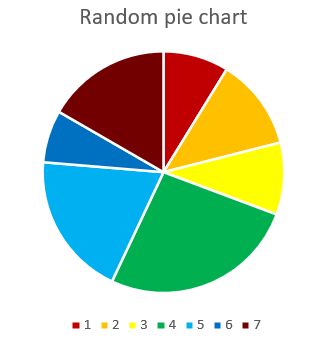
\includegraphics[scale=0.6]{notcolourblindfriendlypiechart.png}
        \end{block}
    \end{column}

    \begin{column}{.5\textwidth}
        \begin{block}{Same piechart simulated for tritanopia (blue-blind)}
            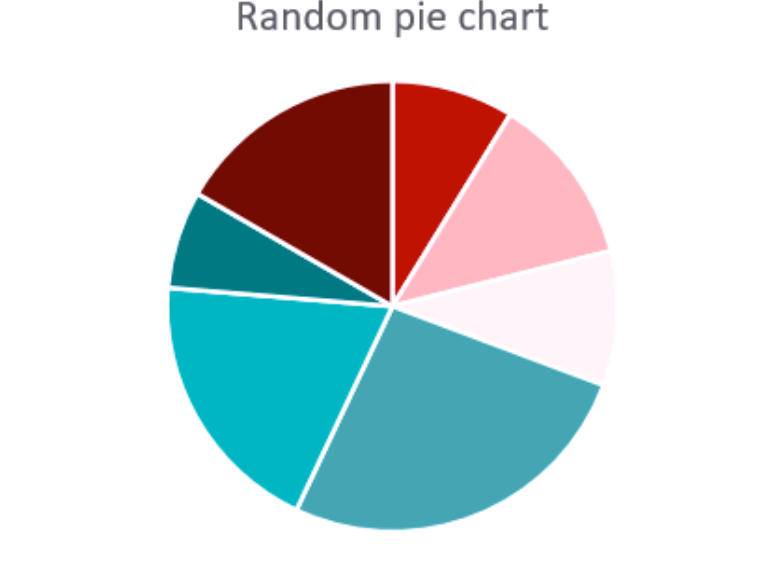
\includegraphics[width=\textwidth]{simulatedpiechart.png}
        \end{block}
    \end{column}

\end{columns}

\end{frame}

\begin{frame}{Colour-blind-friendly graphs}
This is an example of better visuals: a barplot using colour-blind-friendly colours for easy distinction (Data comes from freely available R dataset about states in the USA).
\begin{block}{Real colours}
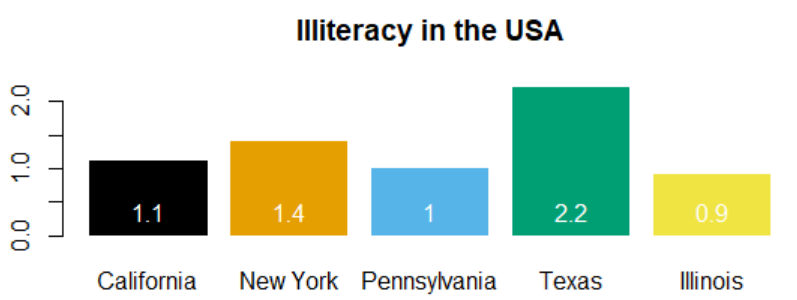
\includegraphics[scale=0.4]{illiteracy in usa.png}
\end{block}

\begin{block}{Same data simulated for tritanopia (blue-blind)}
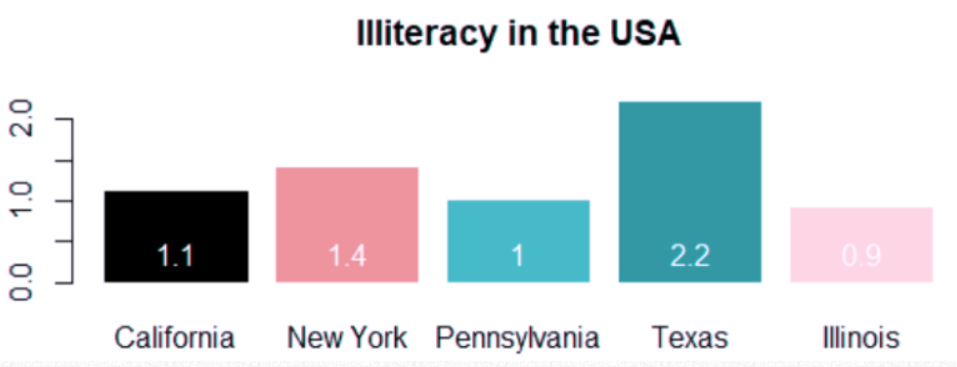
\includegraphics[scale=0.33]{illiteracysimulated.png}
\end{block}
\end{frame}

\begin{frame}{Table made with dcolumn}
\framesubtitle{Aligning the decimal separator}
\begin{table}[ht]
\newcolumntype{a}{D{.}{.}{-1}}
\centering
    \begin{tabular}{aaa}
    \toprule
    \multicolumn{3}{l}{This table was created with \textit{dcolumn}}\\
    \midrule
        -111.00 & 55.40 &  6.50\\
        5555.10 & -0.00001 & 0.011\\
    \midrule
       1.73 & 8.88 & 4.20 \\
       -1.50 & -666.00 & -0.0005 \\
    \bottomrule
    \end{tabular}
    \caption{This meaningless table has all decimal points nicely aligned for easy reading.}
\end{table}
\end{frame}

\begin{frame}{Heatmap}
The net profits of the 5 biggest publicly traded companies in the United States. This visualization quickly makes very clear that Tesla has not been nearly as profitable as other very big companies.
\bigbreak
\begin{table}
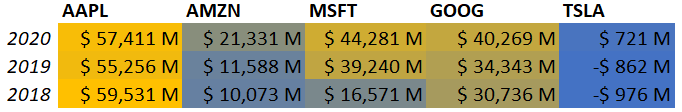
\includegraphics[scale=0.7]{heatmap.png}
\caption{Net Profits for Apple, Amazon, Microsoft, Alphabet and Tesla }
\end{table}
\end{frame}

 \begin{frame}{Colour-blind-friendly graph}
 \begin{figure}[h!]
  \caption{Cumulative stock returns of the 5 biggest US companies, since Nov 23\textsuperscript{rd} 2020.}
   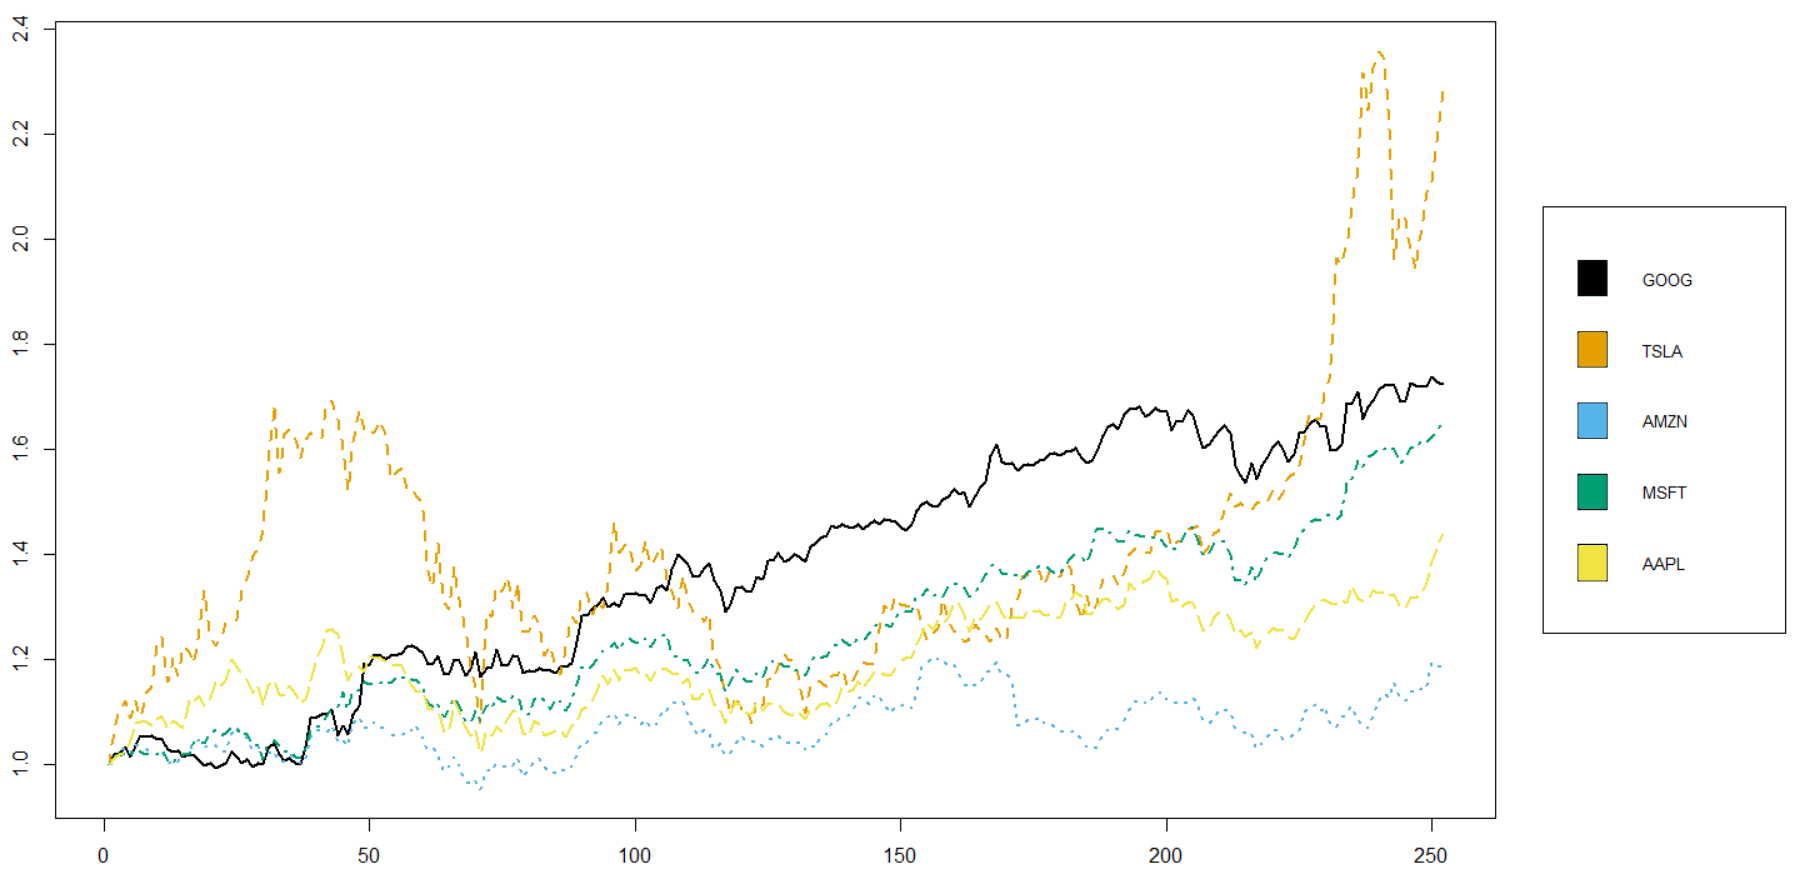
\includegraphics[scale=0.22]{cumreturns.png}
\end{figure}

\end{frame}

\begin{frame}
\printbibliography
\end{frame}

\begin{frame}
\printbibliography
\end{frame}
\end{document}
